

\subsection{Results}\label{M1:results}
In this section we present the results from our numerical simulations. Most of our results concern the evolution of various parameters as a function of $x$. Whenever it's relevant for interpreting and understanding the plot, we mark the point where we have matter-radiation equality and matter-dark energy equality, corresponding to $\om=\orad$ and $\om=\ol$, respectively. These points can be seen directly in \figref{fig:M1:Omegas}. 

\subsubsection{Analytical comparisons \note{(Working title)}}
The dimensionless quantity $\eta\H/c$ is shown in \figref{fig:M1:eta_H_over_c}. At the lowest values of $x\lesssim-10$, we see that $\eta\H/c=1$, as expected. Slightly before matter-radiation equality takes place, we see a slight increase towards higher $x$. As we approach higher $x$, $\ol$ starts dominating, and the solution eventually diverges, as expected. \note{(Comment/derive expression for matter domination?)}.      
\begin{figure}[ht!]
    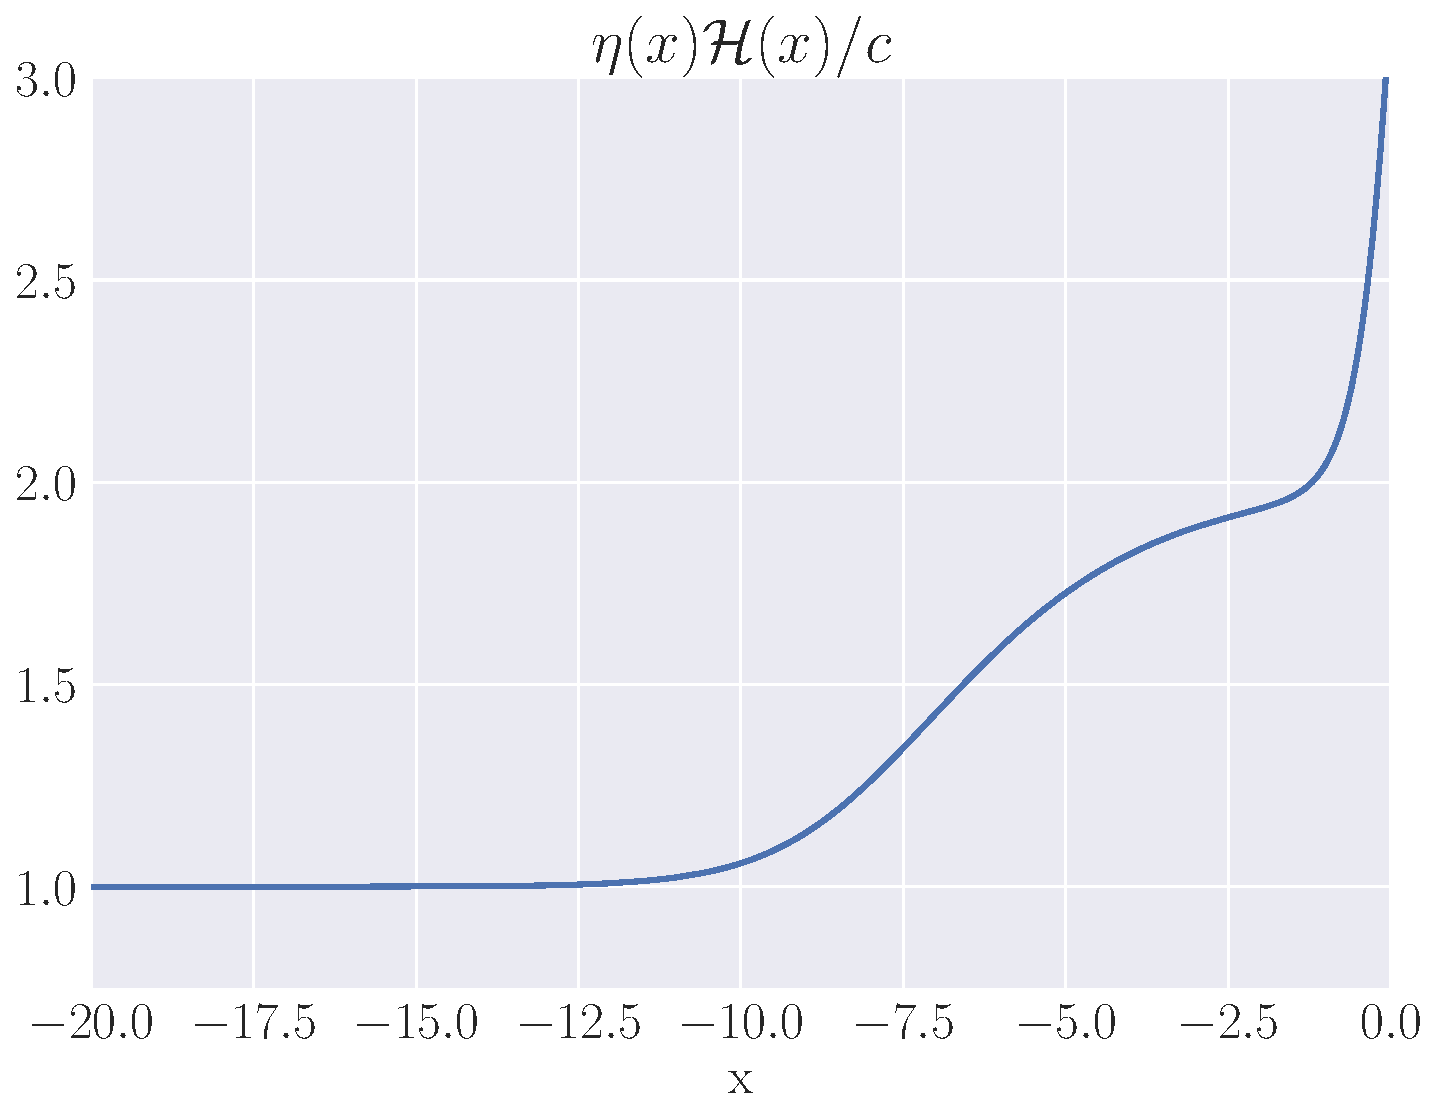
\includegraphics[width=\linewidth]{compare_eta_H_over_c.pdf}
    \caption{Caption}
    \label{fig:M1:eta_H_over_c}
\end{figure}

In \figref{fig:M1:dH_ddH_over_H} we have plotted $\H'/\H$ and $\H''/\H$, where we include the analytical approximation from \eqref{eq:M1:theory:dH_dx_over_H_w} and \eqref{eq:M1:theory:ddH_ddx_over_H_w}, respectively. The different values of $w$ are drawn over the whole range of $x$ where their related density parameter is larger than the other two. This is done for visibility purposes, and we only expect approximations to be reasonable whenever a density parameter is close to $1$. 

Towards the smallest values of $x$ we see that both quantities are well approximated by the analytical solutions for $w=1/3$. As we reach $x\gtrsim12$, matter becomes increasingly dominant, and the solution deviates from being purely dominated by a $w=1/3$ fluid. Towards the highest values of $x$, we see that both quantities reach a constant value of $1$ for $w=-1$. At higher values of $x$, we know that both $\om(x)$ and $\orad(x)$ should vanish, eventually, while $\ol\to1$. This behaviour is thus present in our implementation. When matter is the dominating constituent, we see that neither of the two functions are well approximated by a single fluid with $w=0$ as its equation of state parameter. This can be understood from \figref{fig:M1:Omegas}, where the vanishing contribution of $\orad$ occurs around the same time as $\ol$ starts contributing. The maximum value reached is $\om\approx0.995$. Nonetheless, the deviations are relatively small, and since $\om=1$ is never reached, it's reasonable to assume that our implementations are correct.     
 
\begin{figure}[ht!]
    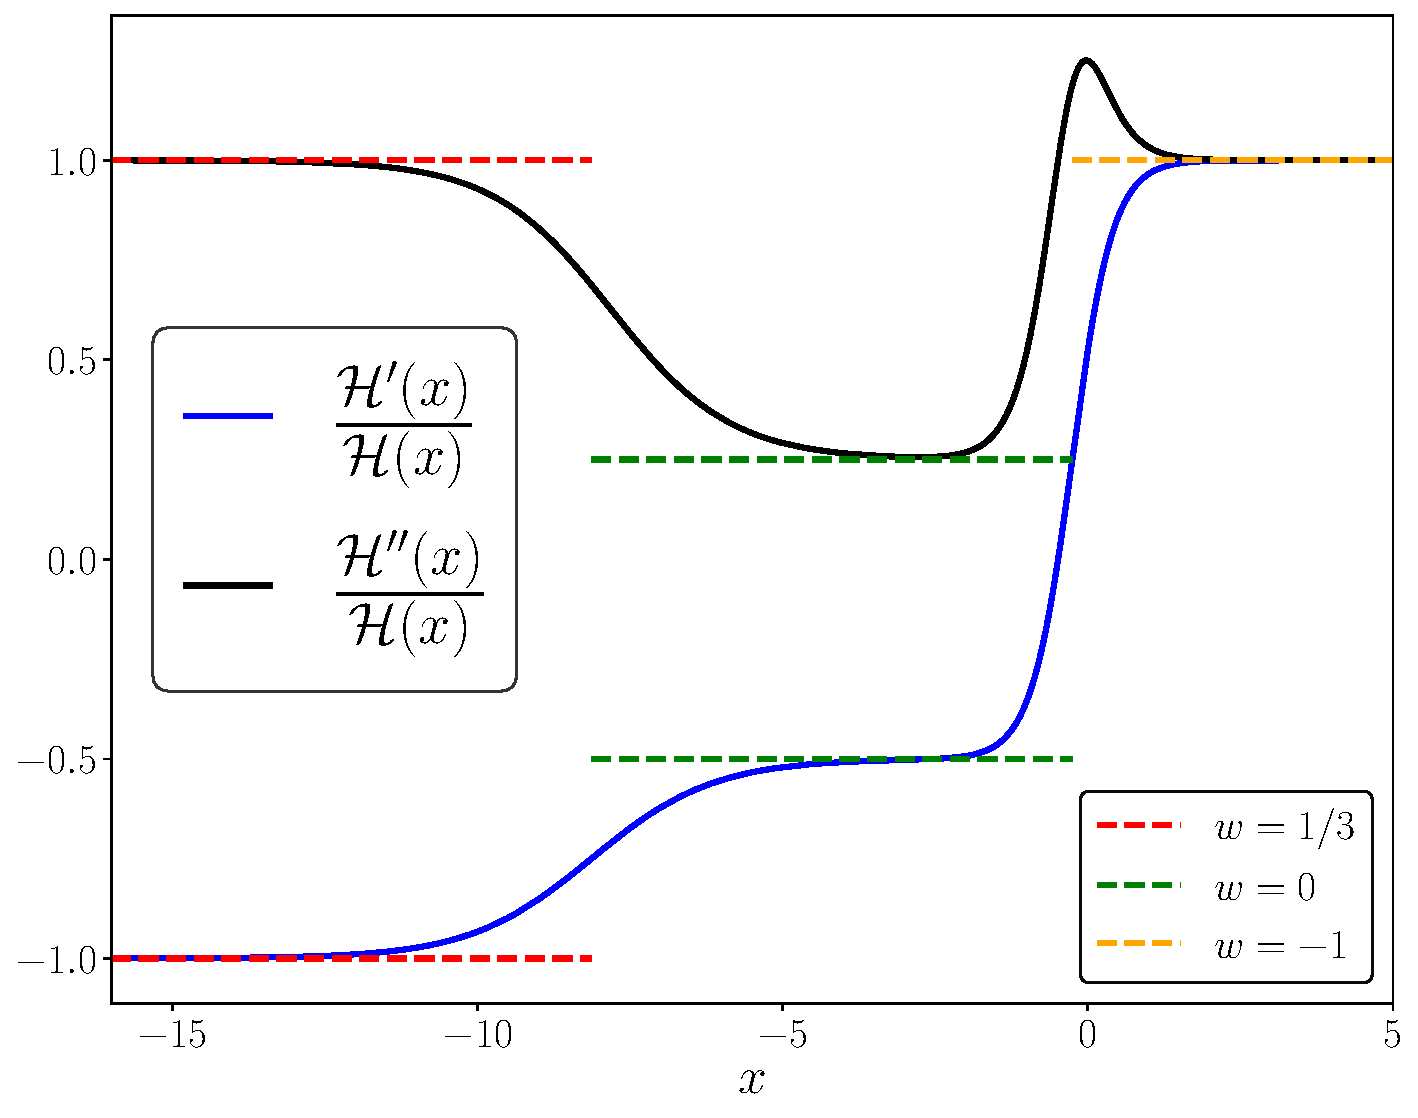
\includegraphics[width=\linewidth]{dH_and_ddH_over_H.pdf}
    \caption{Caption}
    \label{fig:M1:dH_ddH_over_H}
\end{figure}


\subsubsection{Background evolution \note{(working title)}}
Having checked that our implementation is physical, we now proceed by studying the evolution of the background, starting with a plot of the conformal Hubble factor, $\Hx$, show in \figref{fig:M1:Hp_of_x}.

The local minima taking place before matter-dark energy equality corresponds to the onset of acceleration, where $\ddot{a}=0$. For $x>0$, $\ol$ will dominate the conformal Hubble factor, where we have $\Hx\propto e^x$, as seen from Eq. \eqref{eq:M1:theory:Hp_of_x}. 
\begin{figure}[ht!]
    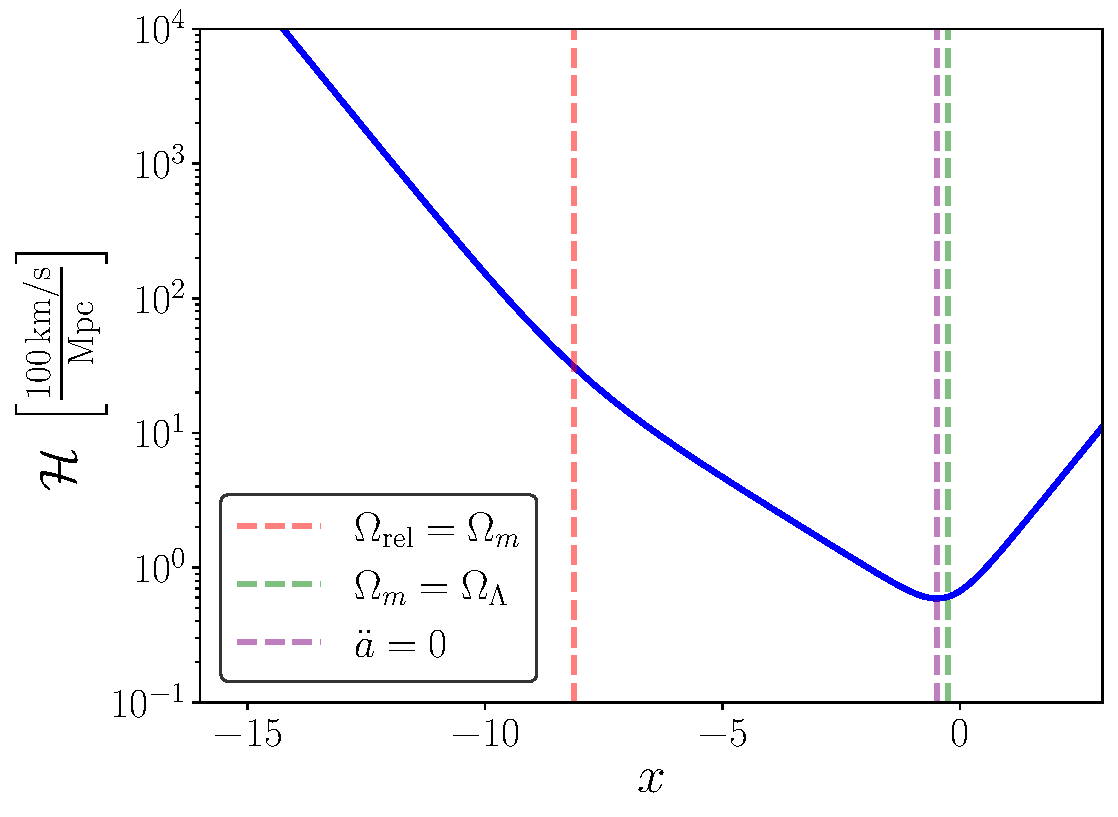
\includegraphics[width=\linewidth]{compare_Hp.pdf}
    \caption{hp}
    \label{fig:M1:Hp_of_x}
\end{figure}

The evolution of $\eta(x)$ and $t(x)$ is shown in \figref{fig:M1:t_and_eta_of_x}. At high values of $x$, the $e^x$ dependence of $\Hx$ causes $\eta(x)$ to grow as $e^{-x}$ at late times, suppressing its growth. The cosmic time, on the other hand, does not have an exponential dependence in the integrand at high values of $x$. This yields the linear growth we see at late times. The different $x$-dependece of $t$ and $\eta$ results in the two quantities to be approximately equal at $x\sim2.75$.    

\note{Include log-plot at early times?}

\begin{figure}[ht!]
    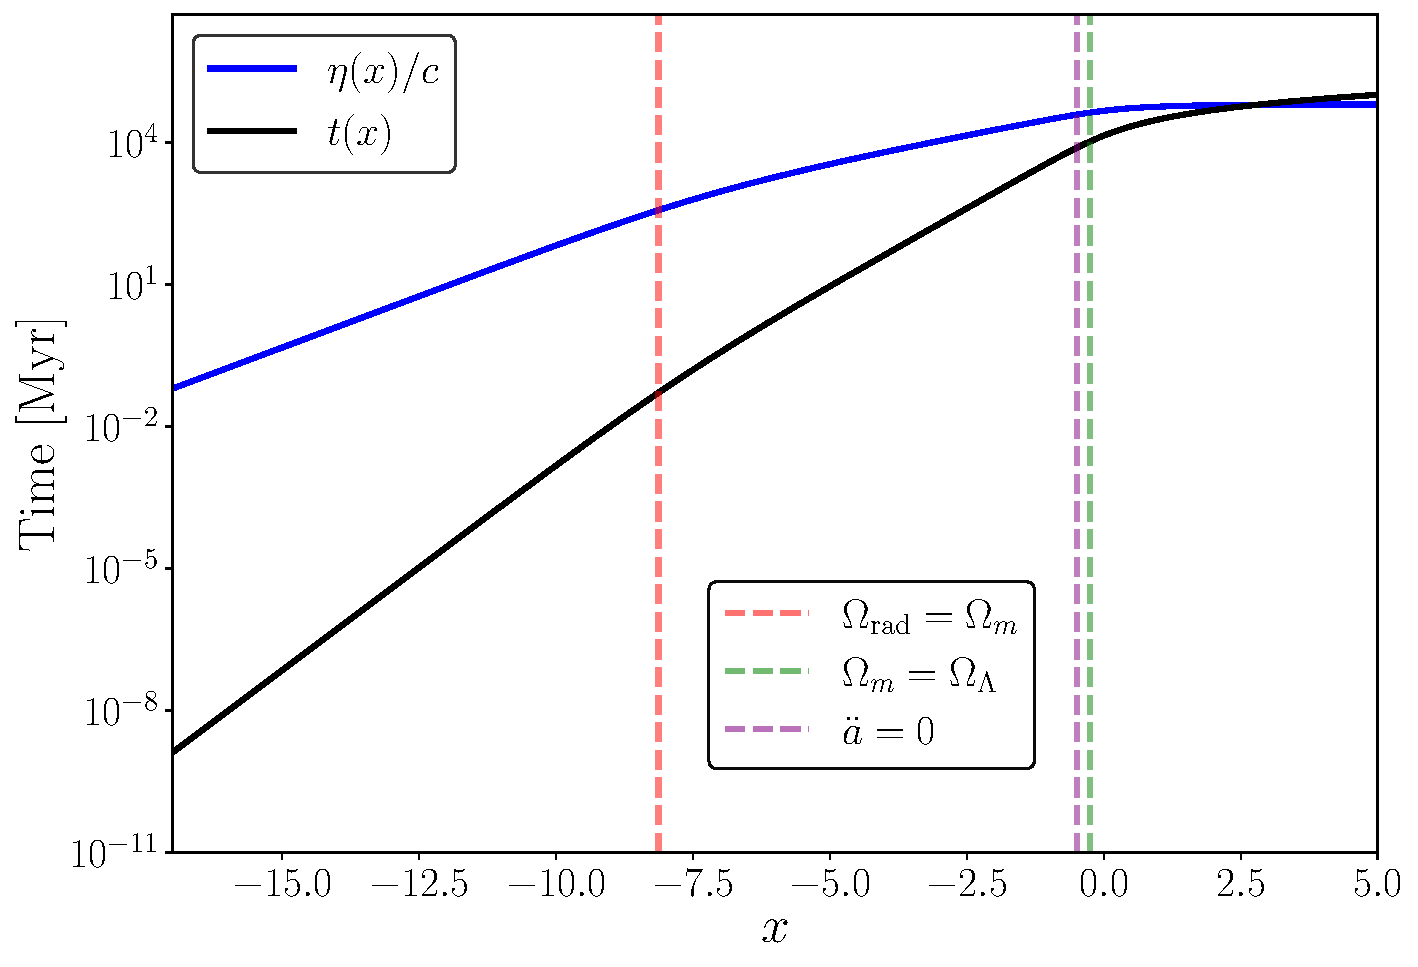
\includegraphics[width=\linewidth]{t_and_eta_c.pdf} 
    \caption{times}
    \label{fig:M1:t_and_eta_of_x}
\end{figure}


\begin{figure}[ht!]
    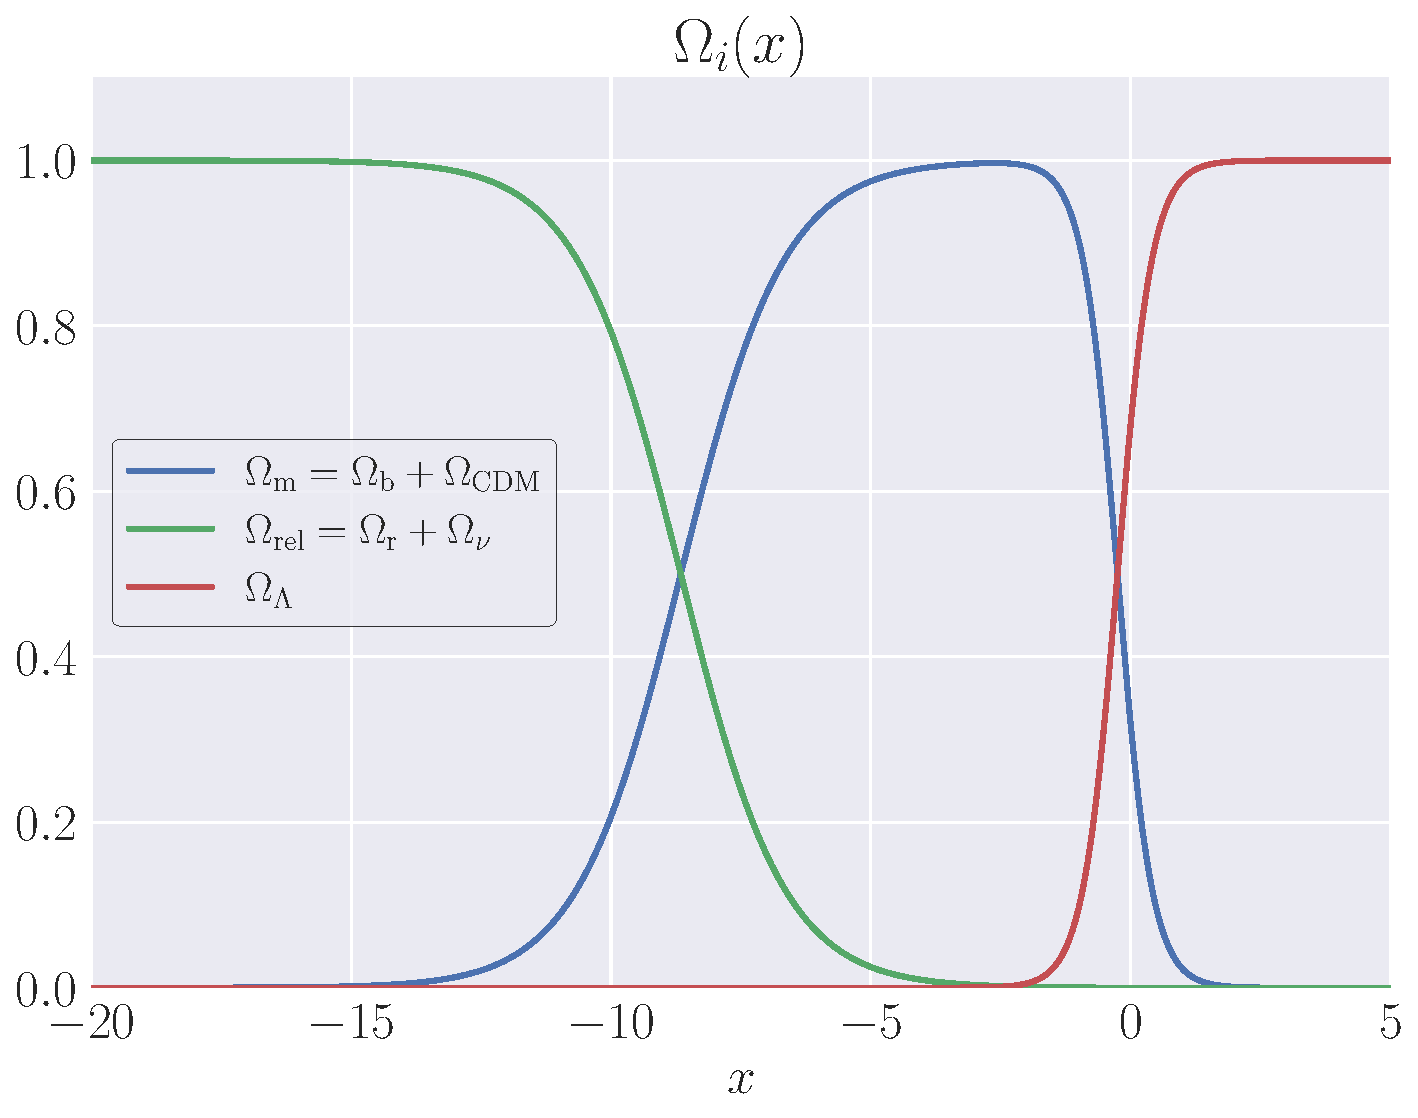
\includegraphics[width=\linewidth]{omega_i_of_x.pdf}
    \caption{Omegas}
    \label{fig:M1:Omegas}
\end{figure}



\subsubsection{Supernova fitting}

A plot showing the luminosity distance as a function of redshift is shown in \figref{fig:M1:dL_of_z_data_vs_Planck}, where we plot $d_L(z)/z$ to better resolve the details \note{(details?)}. There is a noticeable discrepancy between the simulated luminosity distance and the data.      
\begin{figure}[ht!]
    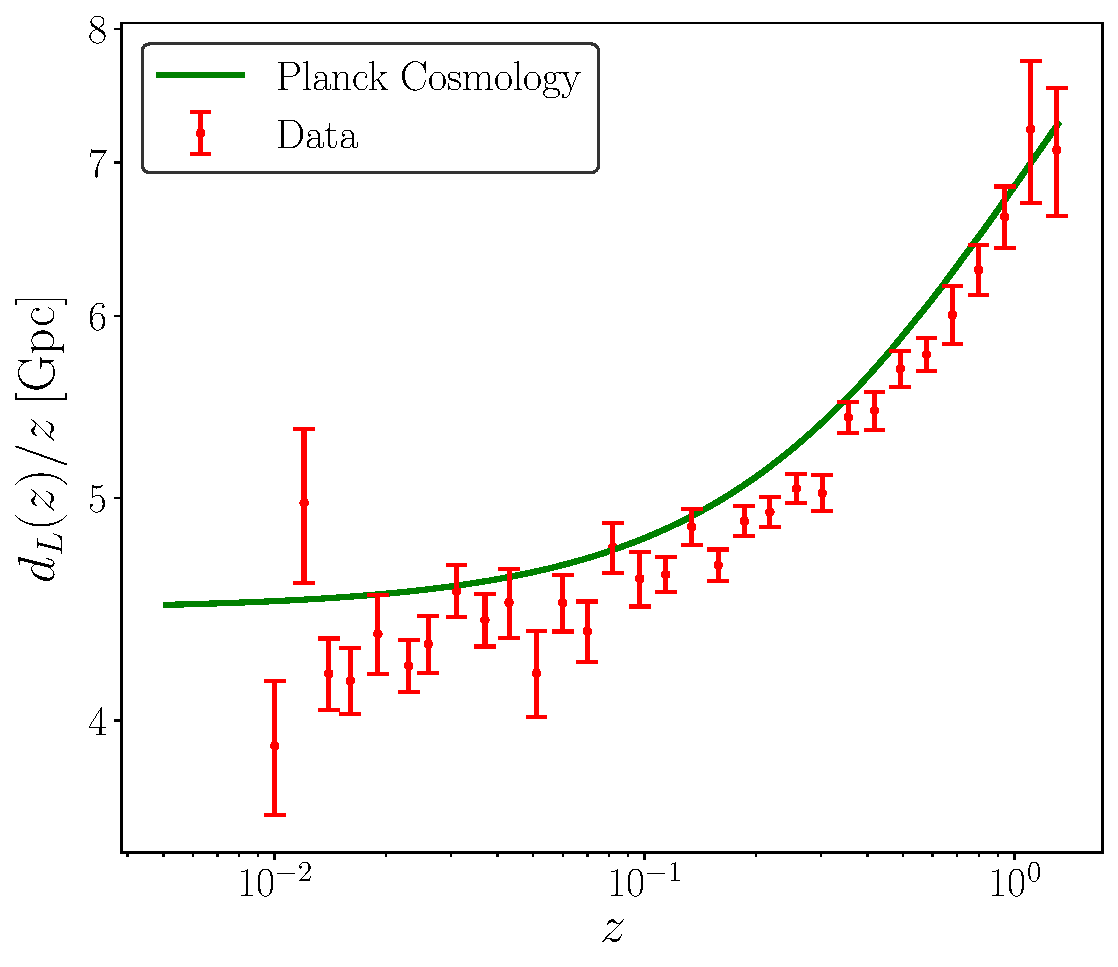
\includegraphics[width=\linewidth]{dL_z_compare_planck.pdf}
    \caption{dlz}
    \label{fig:M1:dL_of_z_data_vs_Planck}
\end{figure}

The $1\sigma$ and $2\sigma$ confidence regions in the $\ol-\om$ plane is shown in \figref{fig:M1:oM_oL_plane}. In the figure we have also indicated the parameter configuration for a flat Universe. A majority of the configurations seem to favour a non-flat Universe, but rather an \note{open} Universe, with $\okn\approx 0.0674$.     
\begin{figure}[ht!]
    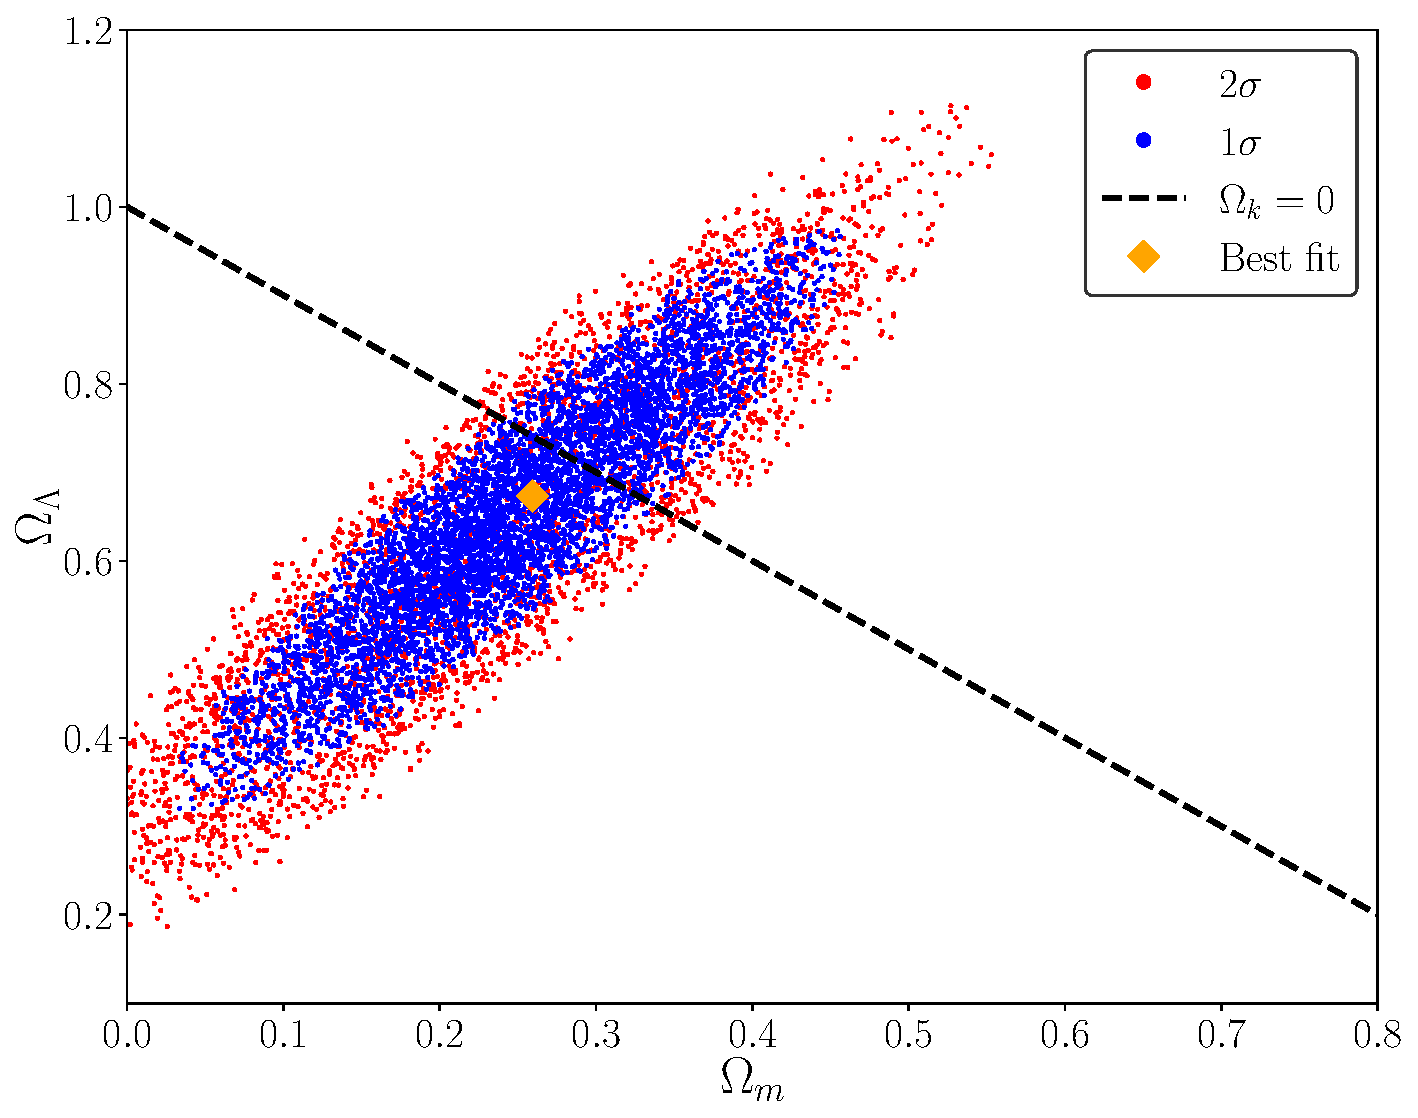
\includegraphics[width=\linewidth]{mcmc_supernova_fit_Nburn1000.pdf}
    \caption{plane}
    \label{fig:M1:oM_oL_plane}
\end{figure}

The posterior PDF of $H_0$ is shown in \figref{fig:M1:H0_posterior_pdf}, where we have included the resulting Gaussian distribution from the mean and variance of the sampled $H_0$ values. This shows further discrepancy from the value of $H_0=67\unit{km/s/Mpc}$, given by Planck, while the mean value we obtain is $\hat{H}_0=70.1\unit{km/s/Mpc}$, with a corresponding standard deviation of $\hat{\sigma}_{H_0}=0.64\unit{km/s/Mpc}$.       
\begin{figure}[ht!]
    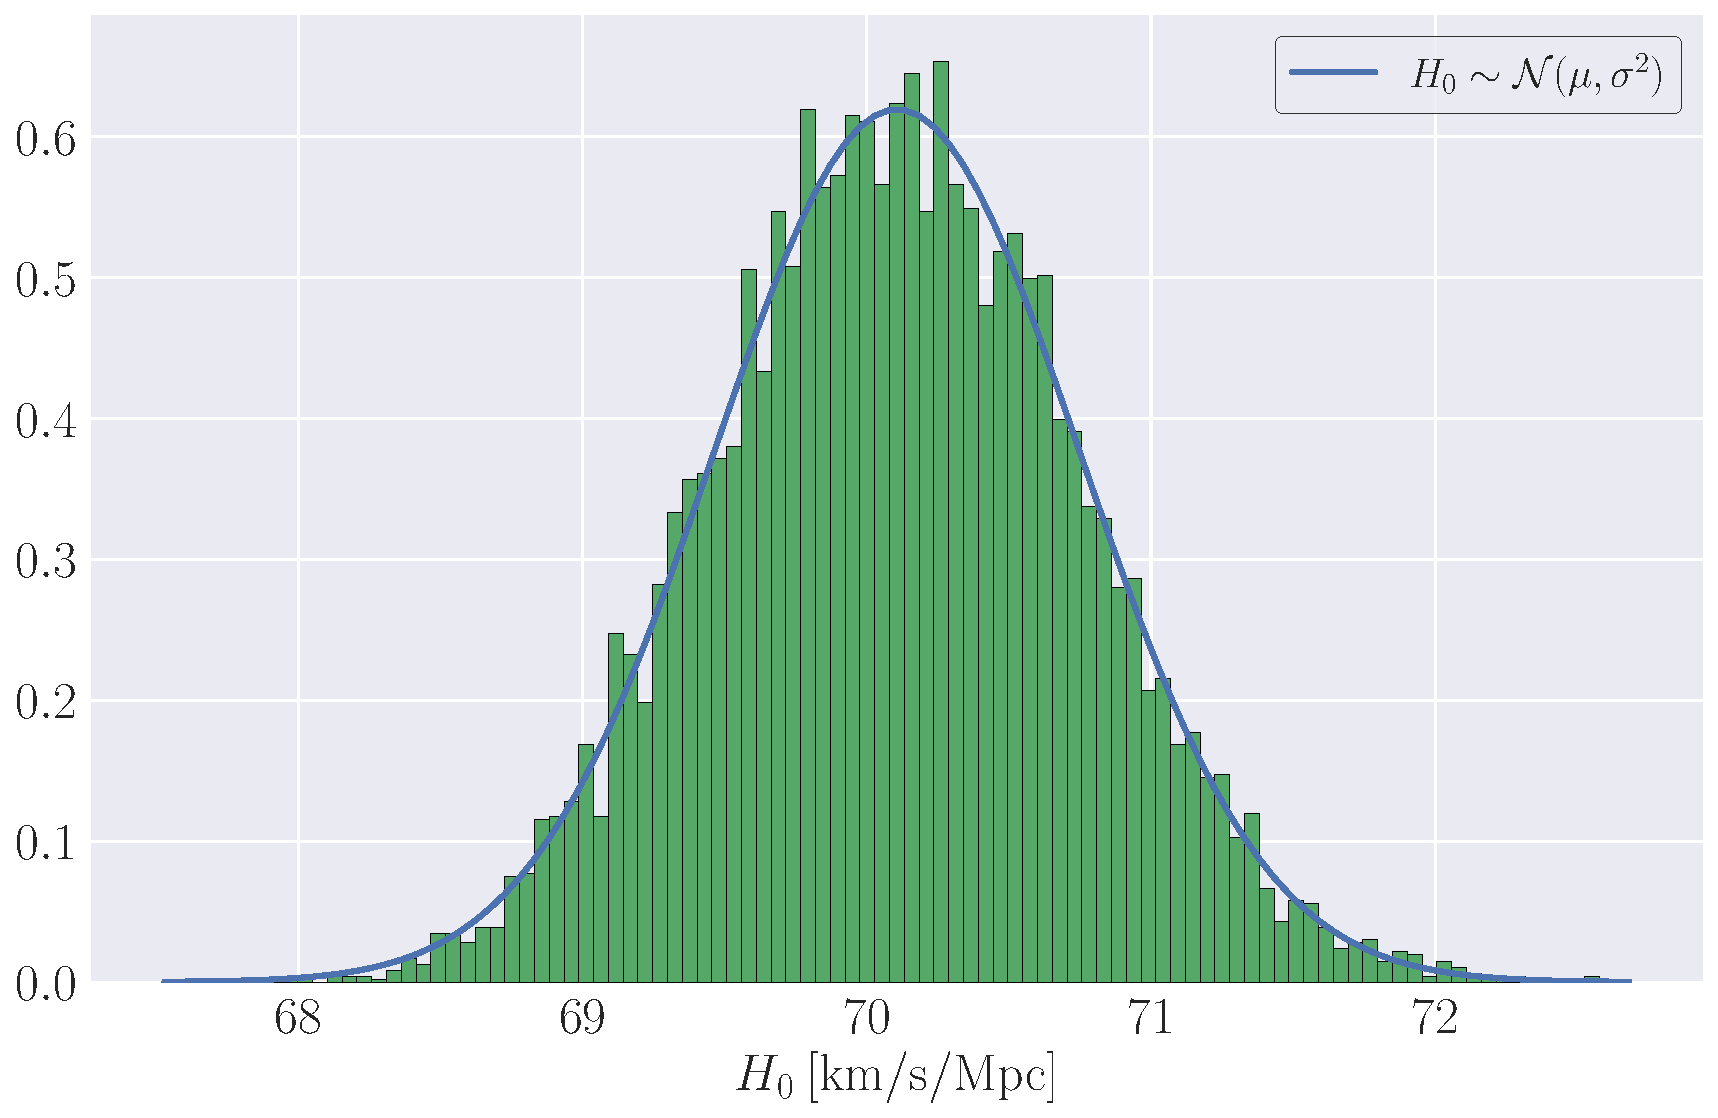
\includegraphics[width=\linewidth]{H0_pdf_Nburn1000.pdf}    
    \caption{pdf}
    \label{fig:M1:H0_posterior_pdf}
\end{figure}


With the fitted parameters, we can solve the background cosmology once again, and compute the resulting luminosity distance  
\begin{figure}[ht!]
    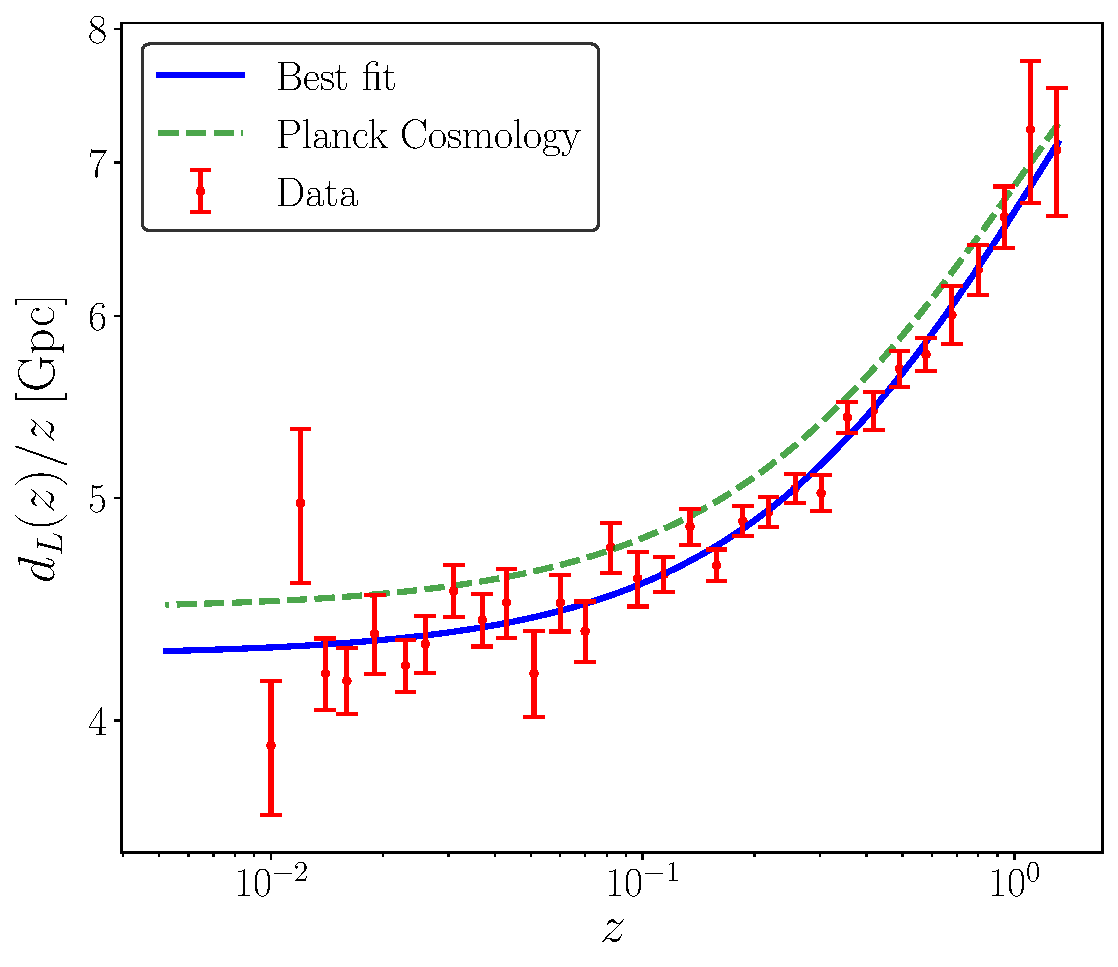
\includegraphics[width=\linewidth]{dL_z_compare_fitted.pdf}
    \caption{dlz}
    \label{fig:M1:dL_of_z_data_vs_bestfit}
\end{figure}

\begin{figure}[ht!]
    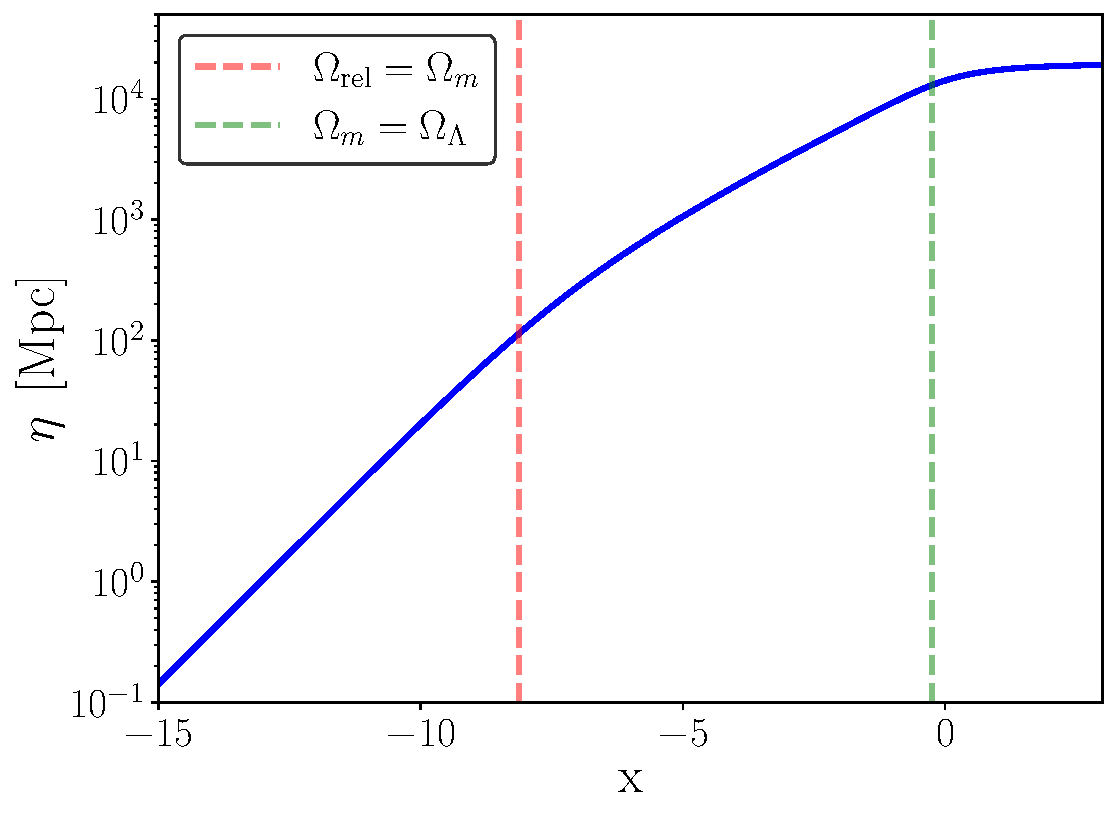
\includegraphics[width=\linewidth]{compare_eta.pdf}
    \caption{\note{REMOVE?}}
    \label{fig:M1:eta}
\end{figure}



% \begin{tabular}{l|ccccc}
\toprule
  & $\Omega_m=\Omega_r$ & $\Omega_m=\Omega_\Lambda$ & $\ddot{a}=0$ & $t_0$ & $\eta_0 / c$ \\
\midrule
$x$ & -8.13 & -0.26 & -0.49 & 13.85 & 46.29 \\
$z$ & 3400.32 & 0.29 & 0.63 & 13.85 & 46.29 \\
$t\unit{Gyr}$ & 51028.91$\unit{yr}$ & 10.37 & 7.75 & 13.85 & 46.29 \\
\bottomrule
\end{tabular}

\begin{tabular}{l|ccccc}
\toprule
  & $\Omega_m=\Omega_r$ & $\Omega_m=\Omega_\Lambda$ & $\ddot{a}=0$ & $t_0$ & $\eta_0 / c$ \\
\midrule
$x$ & -8.13 & -0.26 & -0.49 & 13.85 & 46.29 \\
$z$ & 3400.32 & 0.29 & 0.63 & 13.85 & 46.29 \\
$t\unit{Gyr}$ & 51028.91$\unit{yr}$ & 10.37 & 7.75 & 13.85 & 46.29 \\
\bottomrule
\end{tabular}
